\documentclass[preprintnumbers,amsmath,amssymb,onecolumn,12pt]{revtex4-2}\usepackage{graphicx}% Include figure files
\usepackage{dcolumn}% Align table columns on decimal point
\usepackage{bm}% bold math
\usepackage{natbib}
\usepackage{physics}
\usepackage[caption=false]{subfig}
\newcommand{\be}{\begin{equation}}
\newcommand{\ee}{\end{equation}}

\newcommand{\bea}{\begin{eqnarray}}
\newcommand{\eea}{\end{eqnarray}}
 
\def\sgn{\mathop{\rm sgn}}

\begin{document}
\vspace{0.2in}
{\Large \hspace{1.6in}\textsc{Supplementary Material} }\\
\
\title{Low magnetic field depolarization of NV$^-$ centers through dipole-dipole interaction}

\author{C. Pellet-Mary$^1$, M. Perdriat$^1$, P. Huillery$^?$,  G. H\'etet} 

\affiliation{Laboratoire De Physique de l'\'Ecole Normale Sup\'erieure, \'Ecole Normale Sup\'erieure, PSL Research University, CNRS, Sorbonne Universit\'e, Universit\'e Paris Cit\'e , 24 rue Lhomond, 75231 Paris Cedex 05, France.}

\maketitle

\tableofcontents

\section{NV$^-$ ground state Hamiltonian in low magnetic field}
\label{sec Hamiltonian}
\begin{figure}
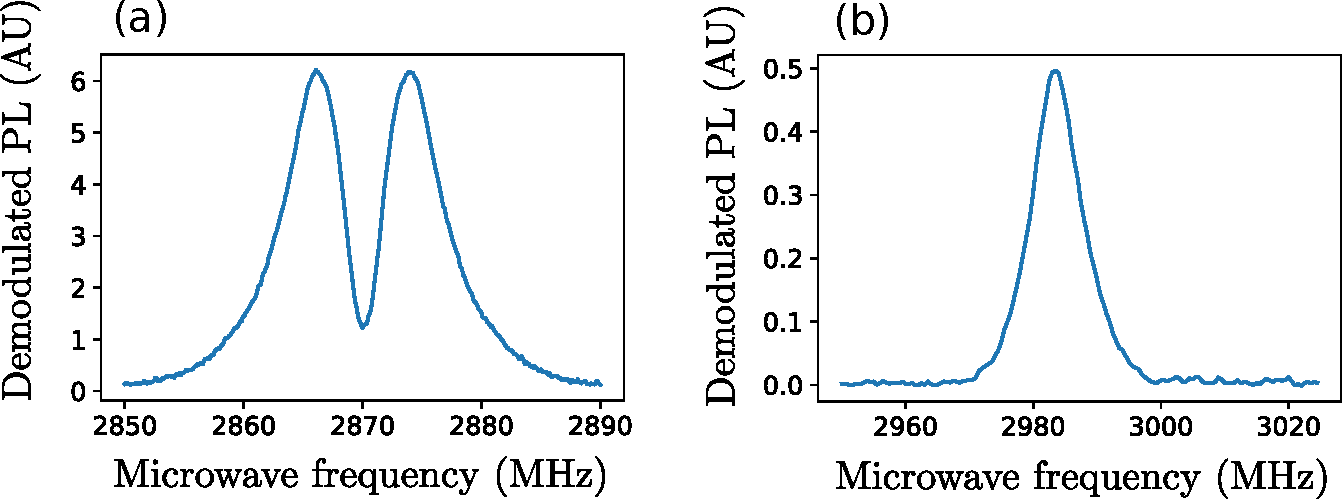
\includegraphics[width=0.9\textwidth]{Figures_SI/fig_ESR}
\caption{ODMR measurement (a) in zero magnetic field, (b) in non-zero magnetic field when zooming on a single class}
\label{ESR_single_spin}
\end{figure}
With zero external magnetic field, there are three possible sources of splitting of the $\{\ket{+1},\ket{-1}\}$ manifold : local electric field, crystal strain and local magnetic field. Of these three causes, only the electric field can explain the shape of the ODMR line that we observe in zero external magnetic field (Fig. \ref{ESR_single_spin}a) \cite{mittiga2018imaging}.

Indeed, random local magnetic field would produce a single broadened line while crystal strain would produce a shifting of the zero field splitting (ZFS) of the same order as the splitting of the levels, which would also blur the two transitions into a single line. On the other hand, due to the large difference between the longitudinal and transverse electric field susceptibilities ($d_\parallel = 0.35\ \rm Hz\, cm/V$ and $d_\perp = 17\ \rm Hz\, cm/V$ \cite{van1990electric}), random local electric field will, on average, cause a splitting much stronger than its ZFS shifting and result in a two peak spectrum.

In our low magnetic field dipole-dipole coupling model, we will therefore neglect the contribution of the strain, local magnetic field and longitudinal electric field.  We also don't take into account the hyper-fine structure of the NV center due to the large inhomogeneous broadening of the transitions (Fig. \ref{ESR_single_spin}b).
We will then consider the following spin Hamiltonian for the NV$^-$ ground state : 
\begin{equation}
\label{NV Hamiltonian}
\mathcal{H}_s=D S_z^2 + \gamma_e \bm{B}_{\rm ext} \cdot \bm{S}+ d_\perp \left[ E_x(S_y^2-S_x^2) + E_y(S_xS_y+S_yS_x) \right]
\end{equation}
Where $D=2.87\ \rm GHz$ is the zero field splitting and $\gamma_e=2.8\ \rm MHz/G$ the gyromagnetic ratio of the electron.

In the absence of an external magnetic field, the symmetry in the ($xy$) plane allows us to chose the $x$ direction along the electric field. The eigenstates of $\mathcal{H}_s$ then become $\{ \ket{0},\ket{+}=\frac{\ket{+1}+\ket{-1}}{\sqrt{2}},\ket{-}=\frac{\ket{+1}-\ket{-1}}{\sqrt{2}} \} $.

In the presence of non-zero magnetic field, let us call the Hamiltonian eigenstates $\{ \ket{g},\ket{d}, \ket{e} \} $. Fig. \ref{map etats propres} shows how close the $\ket{e}$ state is to the $\ket{+1}$ and $\ket{+}$ states as a function of the external magnetic field. Looking at the closeness of $\ket{d}$ to $\ket{-1}$ and $\ket{-}$ would show similar results, while $\ket{g}$ is pretty much equals to $\ket{0}$ for $B<100\ \rm G$.

This tells us that in most cases, the $\{ \ket{0},\ket{+},\ket{-} \}$ basis is only the good Hamiltonian basis for magnetic field smaller than a few Gauss, except in the case of pure transverse magnetic field where the $\{ \ket{0},\ket{+},\ket{-} \}$ basis remains a good basis even for sizable magnetic fields.
\begin{figure}
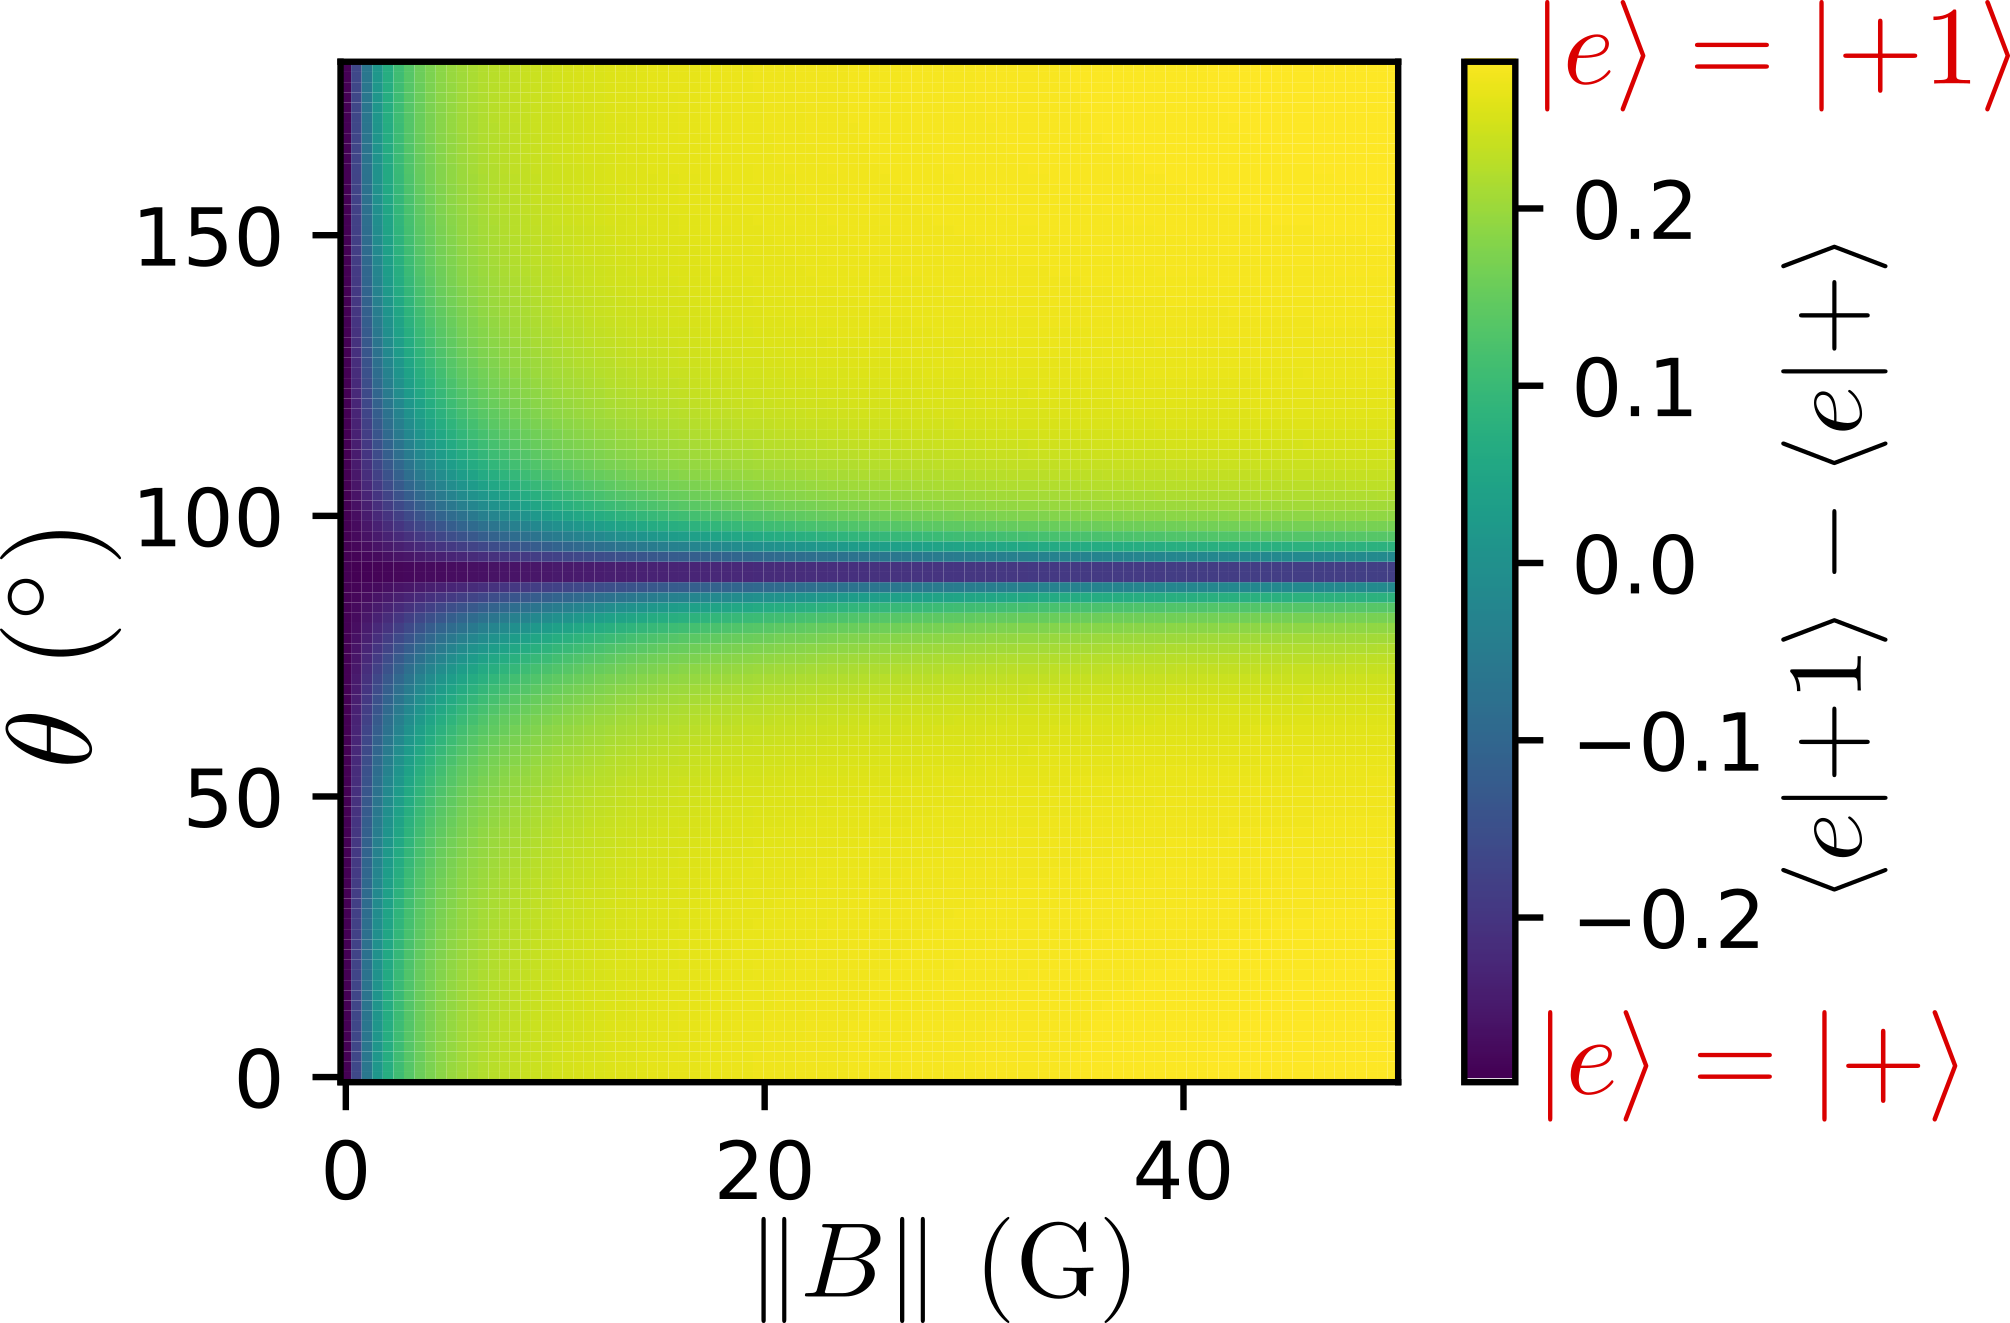
\includegraphics[width=0.7\textwidth]{Figures_SI/map_etats_propres}
\caption{Numerical simulations of the closeness of the Hamiltonian most excited state $\ket{e}$ with the states $\ket{+1}$ and $\ket{+}$, as a function of the magnetic field amplitude and angle $\theta$ with respect to the NV axis. A value of $d_\perp E_\perp = 4\ \rm MHz$ was chosen}
\label{map etats propres}
\end{figure}


\section{Samples}
%Note pour moi : j'ai inversé adamas 1 et 2 parraport aux noms des dossiers dans 20220324
Here are the various samples used in this study :
\begin{itemize}
\item \textbf{HPHT-150-1} : A 150 $\mu$m HPHT 1b diamond irradiated and annealed to reach a concentration [NV$^-$] $\approx 3\ \rm ppm$. Bought as is from Adamas Nanotechnology (MDNV150umHi). This sample is used in Fig. 2 (b), 2(d) and 3 of the main text, as well as Fig. \ref{ESR_single_spin}, \ref{T1_fits} and \ref{alphas} of the SI.
\item \textbf{HPHT-150-2} : Another sample from the same batch as HPHT-150-1. This sample is used in Fig. 4 of the main text and Fig. \ref{largeur_fluct} (c) of the SI.
\item \textbf{HPHT-150-3} : Another sample from the same batch as HPHT-150-1. This sample is used in Fig. \ref{Pola} of the SI.
\item \textbf{HPHT-15-1}  : A 15 $\mu$m diamond with similar properties as the last ones, also bought from Adamas Nanotechnology (MDNV15umHi). This sample is used in Fig. 5 of the main text.
\item \textbf{HPHT-15-2}  : Another sample from the same batch as HPHT-15-1. This sample is used in Fig. \ref{121 VS 22 fig} and \ref{Various ODMR} of the SI.
\item \textbf{CVD-PPM} : A CVD bulk diamond described in \citep{TALLAIRE2020421}. It has been irradiated and annealed and contains [NV$^-$] $\approx 4\ \rm ppm$. This sample is used in Fig. \ref{Alignment} of the SI.
\item \textbf{CVD-PPB} : Another CVD bulk diamond. This one has not been irradiated or annealed and therefore contains [NV$^-$] $\approx 50\ \rm ppb$. This sample is used in Fig. 2(a) of the main text.


\end{itemize}

\section{Experimental Setup}
\begin{figure}
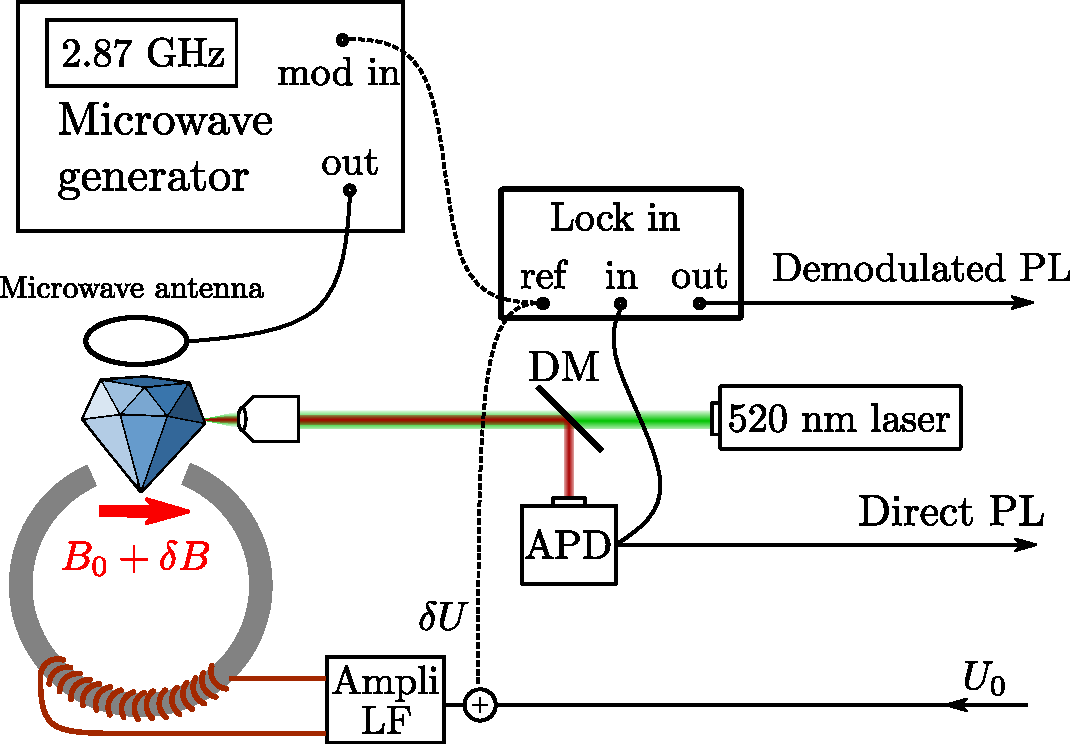
\includegraphics[width=0.7\textwidth]{Figures_SI/shema_exp}
\caption{Experimental Setup}
\label{setup}
\end{figure}
Fig. \ref{setup} shows the general purpose experimental setup used for all the experiments presented in this article.

The optical polarization and readout of the spins is done by focusing a green laser on the diamond sample with an objective lens (NA=0.65), and collecting the back-scattered red fluorescence from the NV center on an avalanche photo-diode (APD, Thorlabs APD410A). The laser is filtered out using a dichroic mirror and a notch filter. The NV$^0$ fluorescence is filtered using an additional 645 nm longpass filter.

The laser used here is a Picoquant PDL 800-D with a 520 nm LDH laser head, providing pulses of 40 ps at a rate of 20 MHz, with an average power of $0.5 \sim 5\ \rm mW$. The trigger of the pulses is generated externally in order to achieve fast  gating of the laser for the $T_1$ measurement. We previously did similar experiment using a continuous 532 nm laser and observed no difference in the behavior of the spins.

The magnetic field is provided by a homemade electromagnet composed of a c-shape iron core and  copper wires. The magnet is mounted on two mechanical rotation stages, allowing a control on the polar and azimuthal angle of the magnetic field within a fraction of a degree and is alimented through a low frequency amplifier (Leybold power function generator 522 63)

The microwave field is generated by a Rhode \& Shwarz SMB 100A and is emitted with a handmade loop antenna. The field is gated by a Mini-circuits ZASWA-2-50DRA+ switch controlled externally and amplified by a Mini-circuits ZHL-5W-422+ amplifier.

A lock-in amplifier (SRS SR830 DSP) is used either to modulate the microwave amplitude for ODMR measurement, or to add an oscillatory magnetic field for the magnetometry protocol. In both case we use a modulation frequency $\sim 1\ \rm kHz$ and demodulate the APD signal.

We did not use magnetic shielding to protect from the earth magnetic field since the splitting due to  $B_{\rm earth}$ is lower than the splitting due to the local electric field for the samples used here : $ \gamma_e B_{\rm earth} \approx 1.5\ \rm MHz < d_\perp E_\perp \approx 4\ \rm MHz$. 
When possible, the electromagnet was roughly aligned along the earth magnetic field to better compensate it.
\section{Experimental details}
\subsection{$T_1$ fitting Protocol}
The $T_1$ profile that we observe with our samples is neither purely exponential, nor purely stretched exponential, which is to be expected when the dipole-dipole spin decay is comparable to the phonon decay.

Fig. \ref{T1_fits} shows the result of a lifetime measurement, measured with the subtraction protocol described in the main text, for zero and non-zero magnetic field. The result is fitted with exponential and stretched-exponential (with a stretch factor $\beta=0.5$) functions. We can see that for the shorter lifetime (zero field), the measurement follows more closely the stretched-exponential profile, while the longer lifetime is closer to the exponential one (except at very short times).

In order to directly compare the results from different magnetic fields, we therefore fit each $T_1$ measurement using both a stretched and exponential decay : $S(\tau)=A \exp (-\frac{\tau}{T_1^{\rm ph}} -\sqrt{\frac{\tau}{T_1^{\rm dd}}})$.
To add consistency to the measurement of $T_1^{\rm dd}$, we fix $T_1^{\rm ph}$ for each sample, leaving $T_1^{\rm dd}$ and the signal amplitude as the only free parameters in the fitting procedure. The value chosen for samples HPHT-150-1 and HPHT-150-2 was $T_1^{\rm ph}=3.62\ \rm ms$. Fig. 1 of the main text shows the result of fitting the same two measurement with this formula.

An other possibility would be to use an arbitrary stretched factor in the fitting function : $S(\tau)=A \exp (-(\frac{\tau}{T_1^{\rm ph}})^\beta )$. Fig. \ref{alphas} shows the optimal $\beta$ parameter as a function of the external magnetic field, which confirms that the $T_1$ profile gets closer to a pure stretched-exponential in zero magnetic field.
\begin{figure}
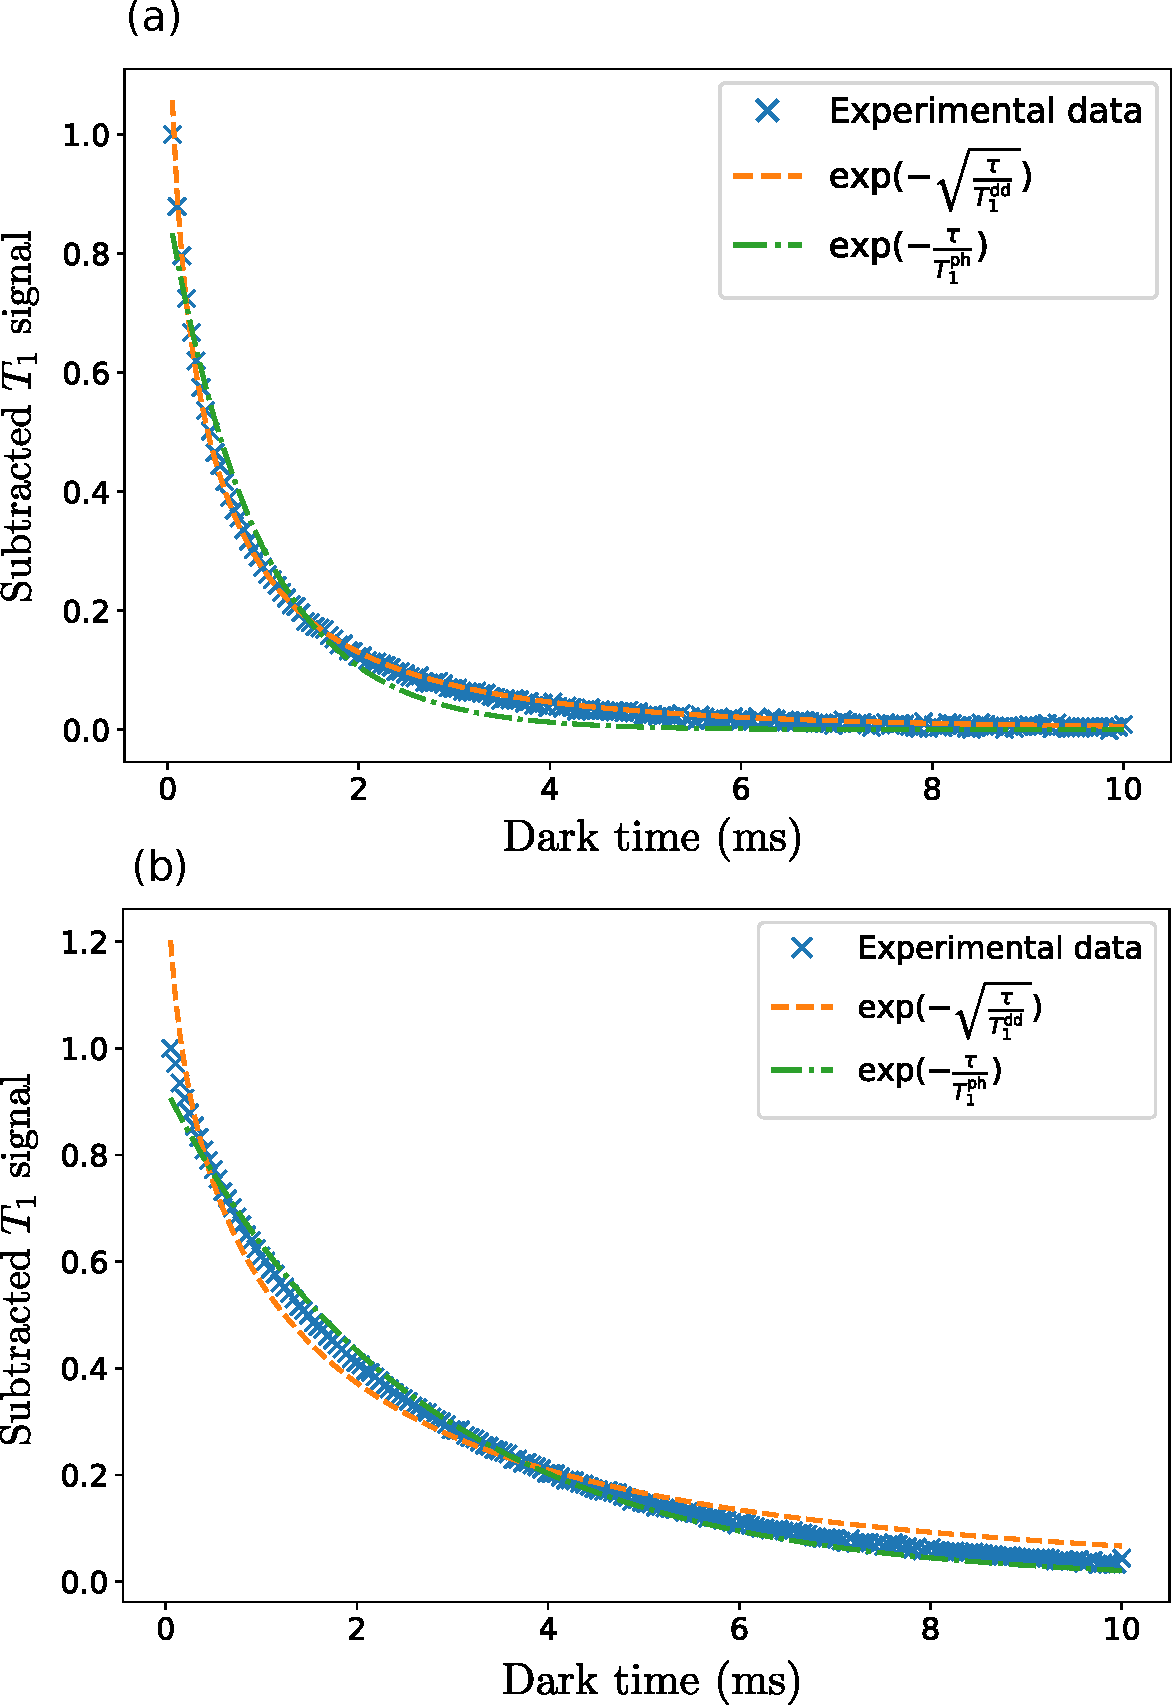
\includegraphics[width=0.8\textwidth]{Figures_SI/Fig_T1_combined}
\caption{$T_1$ measurement with purely exponential and purely stretched exponential fits (a) in zero magnetic field (b) in non-zero magnetic field}
\label{T1_fits}
\end{figure}
\begin{figure}
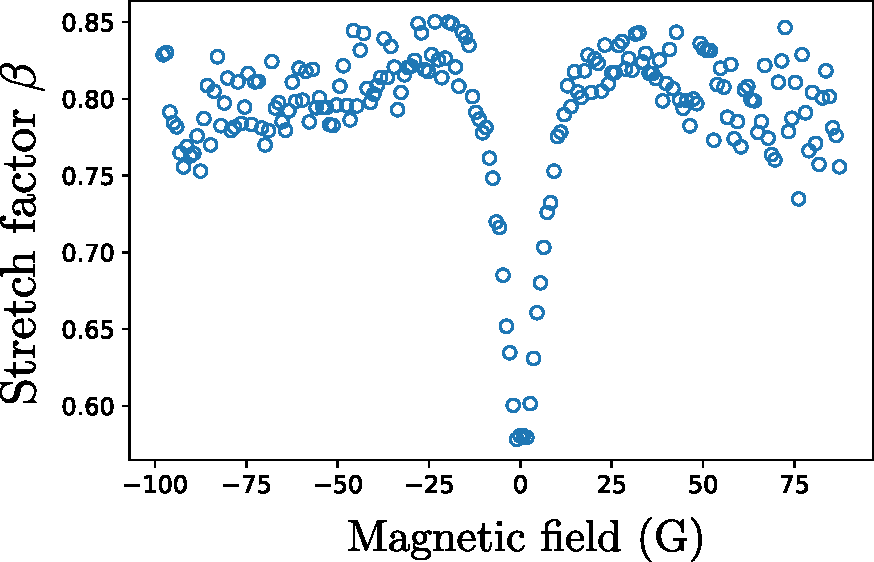
\includegraphics[width=0.45\textwidth]{Figures_SI/fig_alphas}
\caption{Best stretch factor $\beta$ for a $T_1$ fit of the form $f(\tau)=A \exp(-(\frac{\tau}{T_1})^\beta)$ as a function of a randomly oriented magnetic field amplitude}
\label{alphas}
\end{figure}
\subsection{Spectral range of the dipole-dipole cross-relaxations}
\label{fluctuator width}
\begin{figure}
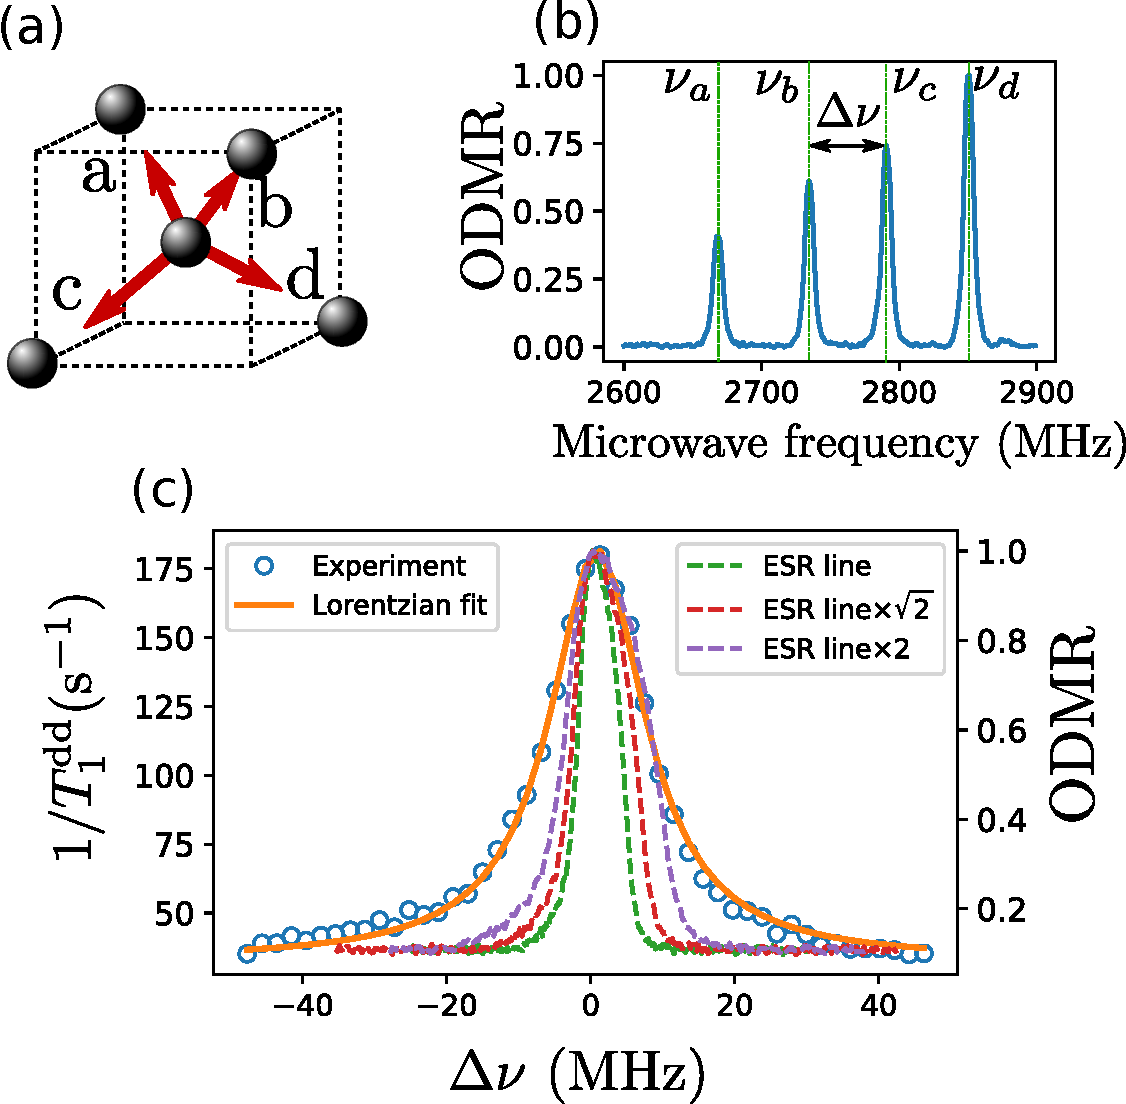
\includegraphics[width=0.7\textwidth]{Figures_SI/largeur_fluct_SI}
\caption{Dipole-dipole depolarization for two near-resonant classes. (a) Sketch of the four possible orientations ("classes") in a single crystal diamond lattice. (b) ODMR spectrum showing four $\ket{0} \to \ket{-1}$ resonances corresponding to the four spin classes. The detuning $\Delta \nu$ between the classes b and c was controlled by changing the orientation of the external magnetic field.(c) Stretch part of the lifetime decay for the spins resonant with $\nu_c$ as a function of the detuning $\Delta \nu$ (blue circles), fitted by a Lorentzian with half width at half maximum 8.04 MHz. Single class ESR line stretched by a factor of 1,$\sqrt{2}$ and 2 are added for comparison}
\label{largeur_fluct}
\end{figure}

An experimental signature of the fluctuator hypothesis developed in \cite{choi_depolarization_2017} is to measure the depolarization rate for two near-resonant classes : if there are indeed very fast decaying NV centers (fluctuators with lifetime $T_1^f < 100 ns$), then the spectral width of the fluctuator would be increased beyond $1/T_2^*$ (which we assume to be homogeneous among all spins in the crystal), which means that they would be able to exchange spin quanta (flip-flop) with non-resonant NV detuned by $\Delta \nu$ such that $2\pi/T_1^f > \Delta \nu > 2\pi/T_2^*$

In order to verify this claim, we have to measure the spectral overlap between two classes, which in the absence of fluctuator should be proportional to the flip-flop rate, and compare it to the actual flip-flop rate which we can measure through the depolarization rate of the spins.

Fig. \ref{largeur_fluct} shows the results of such an experiment where we measured the stretched part of the NV's decay rate, which is very well fitted by a Lorentzian of width $\sigma=8.04 MHz$ (FW or HW ?), and compare it to an ODMR line of a single class of NV centers, stretched by a factor of $\sqrt{2}$ and 2 to simulate the spectral overlap of the two classes (discussed bellow). One should notice that, not only is $1/T_1^{\rm dd}$ significantly larger than the ODMR profile, it also doesn't have the same shape. 

We should note that this broadening can not be explained by the dipole-dipole interaction strength : for a sample with 3 ppm of NV centers, the average dipole-dipole interaction strength between two nearest NV centers $J_0/r^3 \sim 27\ \rm kHz$ which is several order of magnitude lower than the broadening we observe. 

\begin{figure}
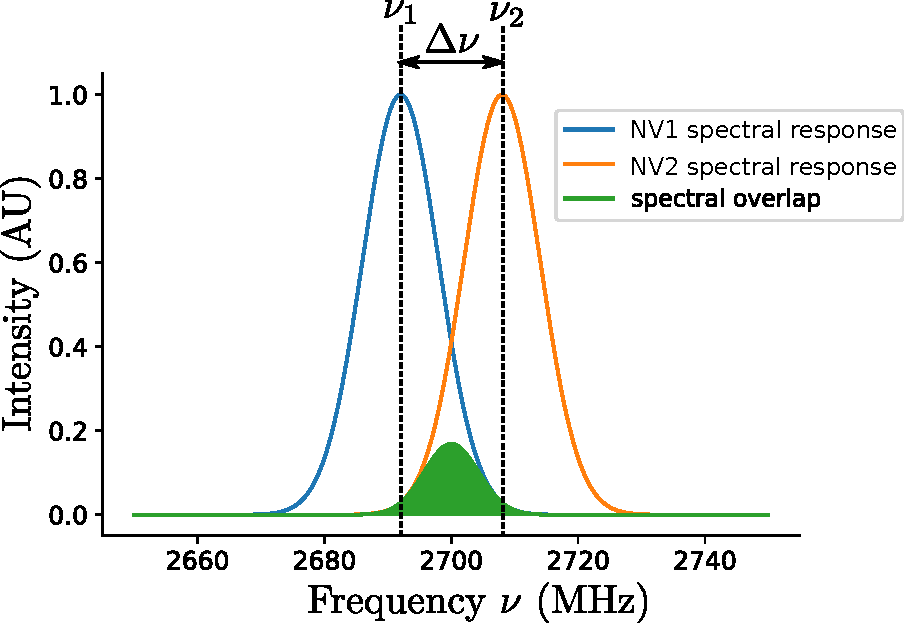
\includegraphics[width=0.7\textwidth]{Figures_SI/overlap}
\caption{Illustration of the spectral overlap for two gaussian spectra}
\label{overlap}
\end{figure}

As illustrated on Fig. \ref{overlap}, we define the spectral overlap $S(\Delta \nu)$ between two spins of spectral response $S_1(\nu)$ and $S_2(\nu)$, centered respectively on the frequencies $\nu_1$ and $\nu_2$ where $\Delta \nu = \nu_2-\nu_1$ as :
\begin{equation}
S(\Delta \nu)=\int S_1(\nu, \nu_1)S_2(\nu, \nu_2) d\nu
\end{equation}
In order to approximate the spectral overlap in our experiment, we will consider the analytical solution in the Gaussian and Lorentzian case :

\begin{itemize}
\item For two gaussians of standard deviation $\sigma$, the spectral overlap as a function of the detuning $\Delta \nu = \nu_1-\nu_2$ is itself a gaussian of standard deviation $\sigma'=\sqrt{2} \sigma$. :
\begin{align*}
S(\Delta \nu)&\propto \int \exp(-\frac{(\nu-\nu_1)^2}{2\sigma^2})\exp(-\frac{(\nu-\nu_2)^2}{2\sigma^2}) d\nu \\
&\propto\exp(-\frac{(\Delta \nu)^2}{4\sigma^2})
\end{align*}

\item For two Lorentzian profile with width $\sigma$, the overlap function is itself a Lorentizan with width $\sigma'=2\sigma$ :
\begin{align*}
S(\Delta \nu)&\propto \int \frac{1}{1+ \frac{(\nu-\nu_1)^2}{\sigma^2}}\cdot \frac{1}{1+ \frac{(\nu-\nu_2)^2}{\sigma^2}} d\nu \\
&\propto\frac{1}{1+ \frac{(\Delta \nu)^2}{4\sigma^2}}
\end{align*}
\end{itemize}

The ODMR lines that we measure are neither Lorentzian nor Gaussian (although they tend to be closer to Gaussians), and can even be asymmetric. Nevertheless, the overlap between two classes can most likely be approximated by a single class ODMR profile stretched by a factor between $\sqrt{2}$ and 2.

\subsection{Lift of the degeneracy between the four classes}

\begin{figure}
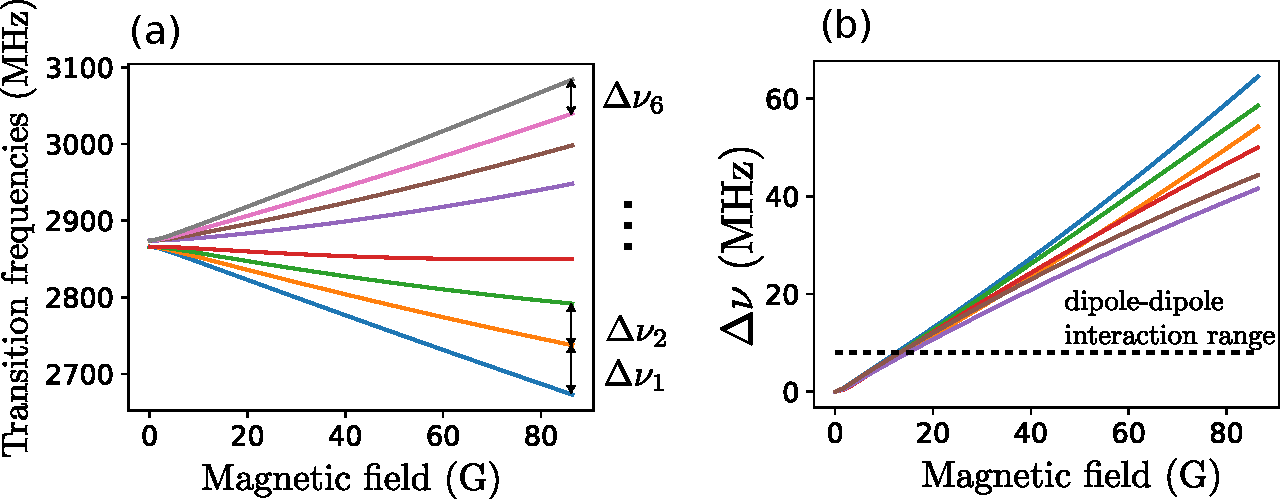
\includegraphics[width=0.9\textwidth]{Figures_SI/Fig_splitting}
\caption{(a) : Simulation of the 8 possible transition frequencies (four $\ket{0} \to \ket{-1}$ and four $\ket{0} \to \ket{+1}$) as a function of the magnetic field amplitude for the orientation of the magnetic field shown in Fig. 3(b) of the main text. (b) Difference in frequency between each pair of closest classes as a function of the magnetic field amplitude. The dotted line y=8.04 MHz correspond to the estimation of the dipole-dipole interaction range.}
\label{splitting}
\end{figure}
We give here an estimate of the magnetic field required to lift the degeneracy of the four classes in the case of Fig. 3(b) of the main text. Fig. \ref{splitting} shows the simulated energies for the 4 $\ket{0} \to \ket{-1}$ and the 4 $\ket{0} \to \ket{+1}$ as a function of the magnetic field, and the difference in energy between the closest pairs of transitions. We can see that the energy detuning between the classes $\Delta \nu$ crosses the value of the dipole-dipole interaction range (8.04 MHz, measured on sample HPHT-150-2 but likely to be similar on sample HPHT-150-1) for magnetic field values $\norm{B} = 12 \sim 15\ \rm G$, which are close to the half-width of the zero-field feature in Fig. 3(b)(ii) and (iii) of the main text.

\subsection{Effect of laser polarization}
Previous studies \cite{anishchik2015low, filimonenko2020weak} reported the presence of a photoluminescence dip in zero magnetic field which was heavily dependent on the laser polarization angle with respect to the diamond axes and the magnetic field. 

We did not observe a strong dependence on the laser polarization with the samples used in this study. Fig.\ref{Pola} shows the photoluminescence from one of our sample as a function of the magnetic field, either directly or with a modulation of the magnetic field, for 6 randomly chosen polarization angle and saw no major difference. 

In particular, we did not observe the apparition of an anti-line inside the main dip, unlike what was observed in the two previously cited work. We expect that the main reason behind the different behaviors is that we seem to observe far grater spin depolarization in zero-field, which we attribute to dipole-dipole coupling, and that this effect could hide smaller effects such as the one related to the laser polarization.
\begin{figure}
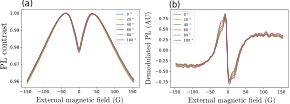
\includegraphics[width=0.9\textwidth]{Figures_SI/fig_Pola}
\caption{Effect of the polarization of the incident laser. (a) Photoluminescence of sample HPHT-150-3 as a function of randomly oriented magnetic field amplitude for various polarization angle. (b) Demodulated PL in the same conditions}
\label{Pola}
\end{figure}
\subsection{Alignment of the magnetic field along [100] axis}
\begin{figure}
\centering
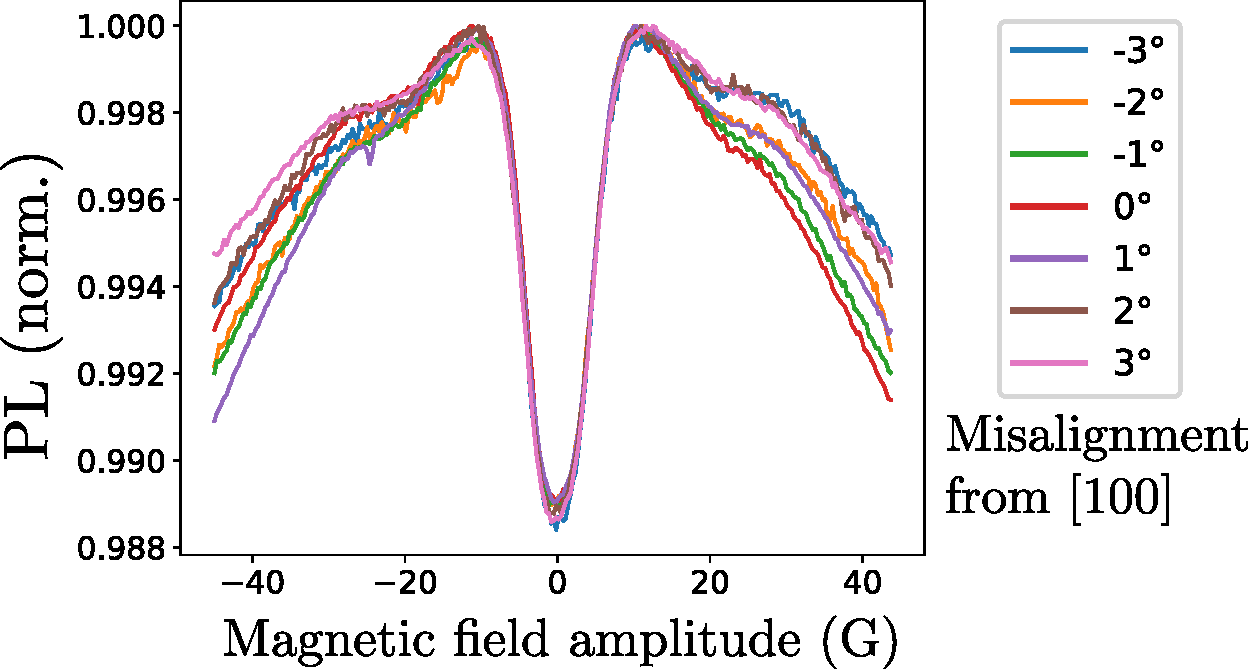
\includegraphics[width=0.6\textwidth]{Figures_SI/alignement}
\caption{PL of sample CVD-PPM as a function of the external magnetic field amplitude for different field misalignment with the [100] axis}
\label{Alignment}
\end{figure}
We claim that the decrease in PL at low magnetic field in Fig. 3 (c)(ii) of the main text is due to to the local electric field and the double flip processes. One other possibility would be a misalignment of the magnetic field with respect to the [100] axis, where the four classes would only be truly resonant with zero external magnetic field.

Fig. \ref{Alignment} shows the change in PL with respect to the external magnetic field amplitude for various misalignment of the magnetic field direction compared to the [100] diamond crystalline axis for sample CVD-PPM. We can see that the central drop in PL is not critically affected by the misalignment of the magnetic field, and we are therefore confident that the drop in PL we observe when $B\parallel [100]$ is not an effect of misalignment.

The initial alignment of the magnetic field was controlled by applying a field of $\sim 50\ \rm G$ and monitoring the overlap of the four classes with ODMR spectra (maximizing the PL drop is also an effective method). We estimate the initial alignment precision to be $\pm 1^\circ$. The misalignment was then added by rotating the electromagnet along an arbitrary axis. The slight asymmetry between the positive and negative value of the magnetic field could come from the earth magnetic field or from hysteresis in the magnetic core of our electromagnet.
\section{Extension of the fluctuator model to low magnetic fields}

\subsection{Results}

Here are the results of the fluctuator model developed in \cite{choi_depolarization_2017} that we extended to include more scenarios. The following sections will detail the calculations that led to these results.
\begin{itemize}
\item The dipole-induced spin decay is at its lowest for a class of NV centers, non resonant with the three other classes, and dominated by a longitudinal magnetic field. In this case the dipole-dipole relaxation is limited by flip-flop processes between spins of the same class. We will call the corresponding stretched lifetime $T_1^{\rm dd}\equiv T_0$.
\item For a single class, still spectrally isolated   from the three other classes, but this time dominated by the electric field or transverse magnetic field (as long as $\gamma_e B_\perp \ll D$), the change in the eigenstates of the single particle Hamiltonian results in an increase of the average flip-flop rate. This leads to a new theoretical stretched lifetime $T_1^{\rm dd}= 4\, T_0$.
\item When a magnetic field is applied along the [100] crystalline axis (for $5\ \rm G < \abs{B} \ll D$), all four classes are resonant and dominated by the longitudinal part of the magnetic field. This results, in increase in the average flip-flop rate compared to the isolated class case, and the predicted stretched exponential lifetime is $T_1^{\rm dd}\approx 42.8\, T_0$.
\item In zero external magnetic field, all four classes are also resonant but we assume that the single particle Hamiltonian of each spin is dominated by a random local electric field. The averaging of flip-flop in this case yields a stretched lifetime $T_1^{\rm dd}\approx 51.4\, T_0$, which is about 20\% higher than the predicted lifetime for $B \parallel$ [100].
\end{itemize}

The effect of the double flip processes was not studied quantitatively since the process is never fully resonant and is therefore highly dependent on the initial splitting of the $\ket{+}$ and $\ket{-} $ states. Nevertheless, the presence of double-flip as an additional relaxation channel can only increase the dipole-induced spin decay rate.

\subsection{Summary of the NV-fluctuator model}
Here are the main hypotheses and conclusion of the NV-fluctuator model developed in \cite{choi_depolarization_2017} :

The NV$^-$ centers in the crystal are divided between two categories : "normal" NV centers (simply called NV) which, in the absence of dipole-dipole coupling would have a phonon-limited $T_1$ ($T_1^{NV}\sim \rm ms$), and fluctuators who are NV centers with an additional, fast, depolarization mechanism, such that their lifetime $T_1^f < 100\ \rm ns$. Having such a short lifetime, the fluctuators are almost unpolarized by the green laser, making them invisible in standard optical NV measurement protocol ($T_1$, ODMR, etc.). 

Assuming a homogeneous distribution of the fluctuators in the bulk of the crystal, the authors of \cite{choi_depolarization_2017} conclude that the fluctuators create an additionnal decay channel for the NV population, through dipole-dipole interaction, characterized by a decay rate $\gamma$ which follows the probability distribution :
\begin{equation}
\rho(\gamma)=\frac{e^{-1/(4\gamma T)}}{\sqrt{4\pi \gamma^3 T}}
\end{equation}
Where the timescale $T$ is defined as
\begin{equation}
\frac{1}{T}=\left(\frac{4\pi n_fJ_0\bar \eta}{3}\right)^2 \frac{\pi}{\gamma_f}
\label{eq 1/T}
\end{equation}
Where $n_f$ is the fluctuator density in the crystal in nm$^{-3}$, $J_0=52\ \rm{MHz}\cdot\rm{nm}^3$ is the characteristic dipole-dipole strength between two spins, $\gamma_f$ is the fluctuator intrinsic decay rate and $\bar \eta$ is a dimension-less number which characterizes the average dipole-dipole interaction between the NV centers and the fluctuators (resonance conditions, relative orientations etc. Further details are given below).

The polarization dynamics of the averaged ensemble of NV centers then follows :
\begin{equation}
P(t)=\int_0^\infty \rho(\gamma)\, e^{-\gamma t}d\gamma= e^{-\sqrt{t/T}}
\end{equation}
Which corresponds to the stretched-exponential part of the lifetime measurement.
\subsection{Dipole-Dipole Hamiltonian between two NV$^-$ centers}
We consider a system composed of an NV center interacting dipolarly with a fluctuator.
\begin{equation}
\mathcal{H}_{\rm tot}=\mathcal{H}_{1}+\mathcal{H}_2+\mathcal{H}_{\rm dd}
\end{equation}
Where $\mathcal{H}_{1}$ and $\mathcal{H}_{2}$ are the single particle Hamiltonian of the NV and fluctuator, described by the equation (\ref{NV Hamiltonian}), and $\mathcal{H}_{\rm dd}$ is the dipole-dipole interaction Hamiltonian between the two spins. 

We will consider the spin operators $\bm{S}_1$ and
$\bm{S}_2$ in the NV own basis : the $z$ orientation of the $S_z$ operator is chosen along the NV axis of each spin. In the presence of a longitudinal magnetic field, the sense of $\hat{z}$ will be chosen such that $\bm{B}\cdot \hat{z} >0$, and the $\hat{x}$ direction is chosen along the transverse magnetic or electric field, whichever dominates the single spin Hamiltonian. These choices mean that there will be two distinct Cartesian basis $\{\hat{x}_1,\hat{y}_1,\hat{z}_1\}$ and $\{\hat{x}_2,\hat{y}_2,\hat{z}_2\}$ describing the two spins.

The dipole-dipole Hamiltonian can then be decomposed as :
\begin{align}
-\frac{\mathcal{H}_{\rm dd}}{J_0/r^3}&= 3\left({\bm S}_1 \cdot \hat{u} \right)\left({\bm S}_2 \cdot \hat{u} \right) - {\bm S}_1 \cdot {\bm S}_2  \\
&=\left[3(\hat{u}\cdot\hat{x}_1)(\hat{u}\cdot\hat{x}_2) -\hat{x}_1\cdot\hat{x}_2\right] S_x^1S_x^2 \\
&+\left[3(\hat{u}\cdot\hat{y}_1)(\hat{u}\cdot\hat{y}_2) -\hat{y}_1\cdot\hat{y}_2\right] S_y^1S_y^2 \\
&+\left[3(\hat{u}\cdot\hat{x}_1)(\hat{u}\cdot\hat{y}_2) -\hat{x}_1\cdot\hat{y}_2\right] S_x^1S_y^2 \\
&+\left[3(\hat{u}\cdot\hat{y}_1)(\hat{u}\cdot\hat{x}_2) -\hat{y}_1\cdot\hat{x}_2\right] S_y^1S_x^2 \\
&+\left[3(\hat{u}\cdot\hat{z}_1)(\hat{u}\cdot\hat{z}_2) -\hat{z}_1\cdot\hat{z}_2\right] S_z^1S_z^2 \\
&+\mathcal{H}_{\rm other}
\end{align}
Where $J_0=\frac{\mu_0 \gamma_e^2 \hbar^2}{4 \pi} = (2 \pi) 52\ \rm MHz \cdot \rm{nm}^3$, $\bm r= r\bm{\hat u}$ is the distance between the two spins and  $\mathcal{H}_{\rm other}$ contains terms of the form $S_{x/y}^iS_z^j$ which couple states far from resonance and will be neglected here.

\subsection{Flip-flops in the magnetic basis $\{ \ket{0},\ket{+1},\ket{-1} \} $}
We will first consider the case, treated in \cite{choi_depolarization_2017}, where the longitudinal magnetic field is strong enough that the single spin Hamiltonian eigenstates of both spins are close to $\{ \ket{0},\ket{+1},\ket{-1} \} $ (since we are interested in near-resonant spins, this means that both spins see roughly the same longitudinal and transverse magnetic field).

In this scenario, only flip-flop terms (that is $\mel{\pm 1,0}{\mathcal{H}_{\rm dd}}{0,\pm 1}$) can couple two resonant two-spins states. Following the notation in \cite{choi_depolarization_2017}, we introduce the dimensionless factor $\eta$ defined as : 
\begin{equation}
\eta^2=\frac{1}{3} \abs{\mel{\pm 1,0}{\frac{\mathcal{H}_{\rm dd}}{J_0/r^3}}{0,\pm 1}}^2  \frac{4\gamma_f^2}{(\omega_f - \omega_{NV})^2+4\gamma_f^2}
\end{equation}
Where $\gamma_f$ is the fluctuator lifetime, $\omega_f$ the fluctuator angular frequency and $\omega_{NV}$ the NV angular frequency. %This numerical factor characterizes both the dipole-dipole strength between the NV and the fluctuator through the matrix element and the resonance condition through the Lorentzian function.

This numerical factor is linked to the previously mentioned $\bar \eta$ by averaging over every possible orientation and angular position of the fluctuators. Assuming that the fluctuators are evenly distributed among all four classes (NV axis orientation) and decomposing the $\bm r$ vector in the spherical basis ($r, \theta, \phi$), we can write $\bar \eta$ as :

\begin{equation}
\label{eq. eta bar}
\bar \eta =\frac{1}{4} \sum_{i=1}^4 \int_\theta \int_\phi  \int_{\omega_f} \int_{\omega_{NV}}   \abs{\eta(\bm u,i,\omega_{NV},\omega_f)}\, d\Omega\, \rho(\omega_{NV}) d\omega_{NV}\, \rho^i(\omega_f) d\omega_f 
\end{equation}

Where $d\Omega=\sin \theta d\theta d\phi$, $\rho(\omega_{NV})$ is the distribution of angular frequencies of the probed NV centers, and  $\rho^i(\omega_f)$ is the distribution of angular frequencies  for the fluctuators of class $i$.

While the distributions $\rho(\omega_{NV})$ and $\rho^i(\omega_f)$ can be approximated using the data presented in Fig. \ref{largeur_fluct}, we will assume that these distributions are independent of the external magnetic field, and since we are interested in comparing the same sample for various values of the magnetic field, we will simplify eq.(\ref{eq. eta bar}) by postulating that $\frac{4\gamma_f^2}{(\omega_f - \omega_{NV})^2+4\gamma_f^2} =1$ if the NV center's and the fluctuator's classes are resonant (or if they are from the same class), and $\frac{4\gamma_f^2}{(\omega_f - \omega_{NV})^2 +4\gamma_f^2}=0$ otherwise.

\begin{figure}
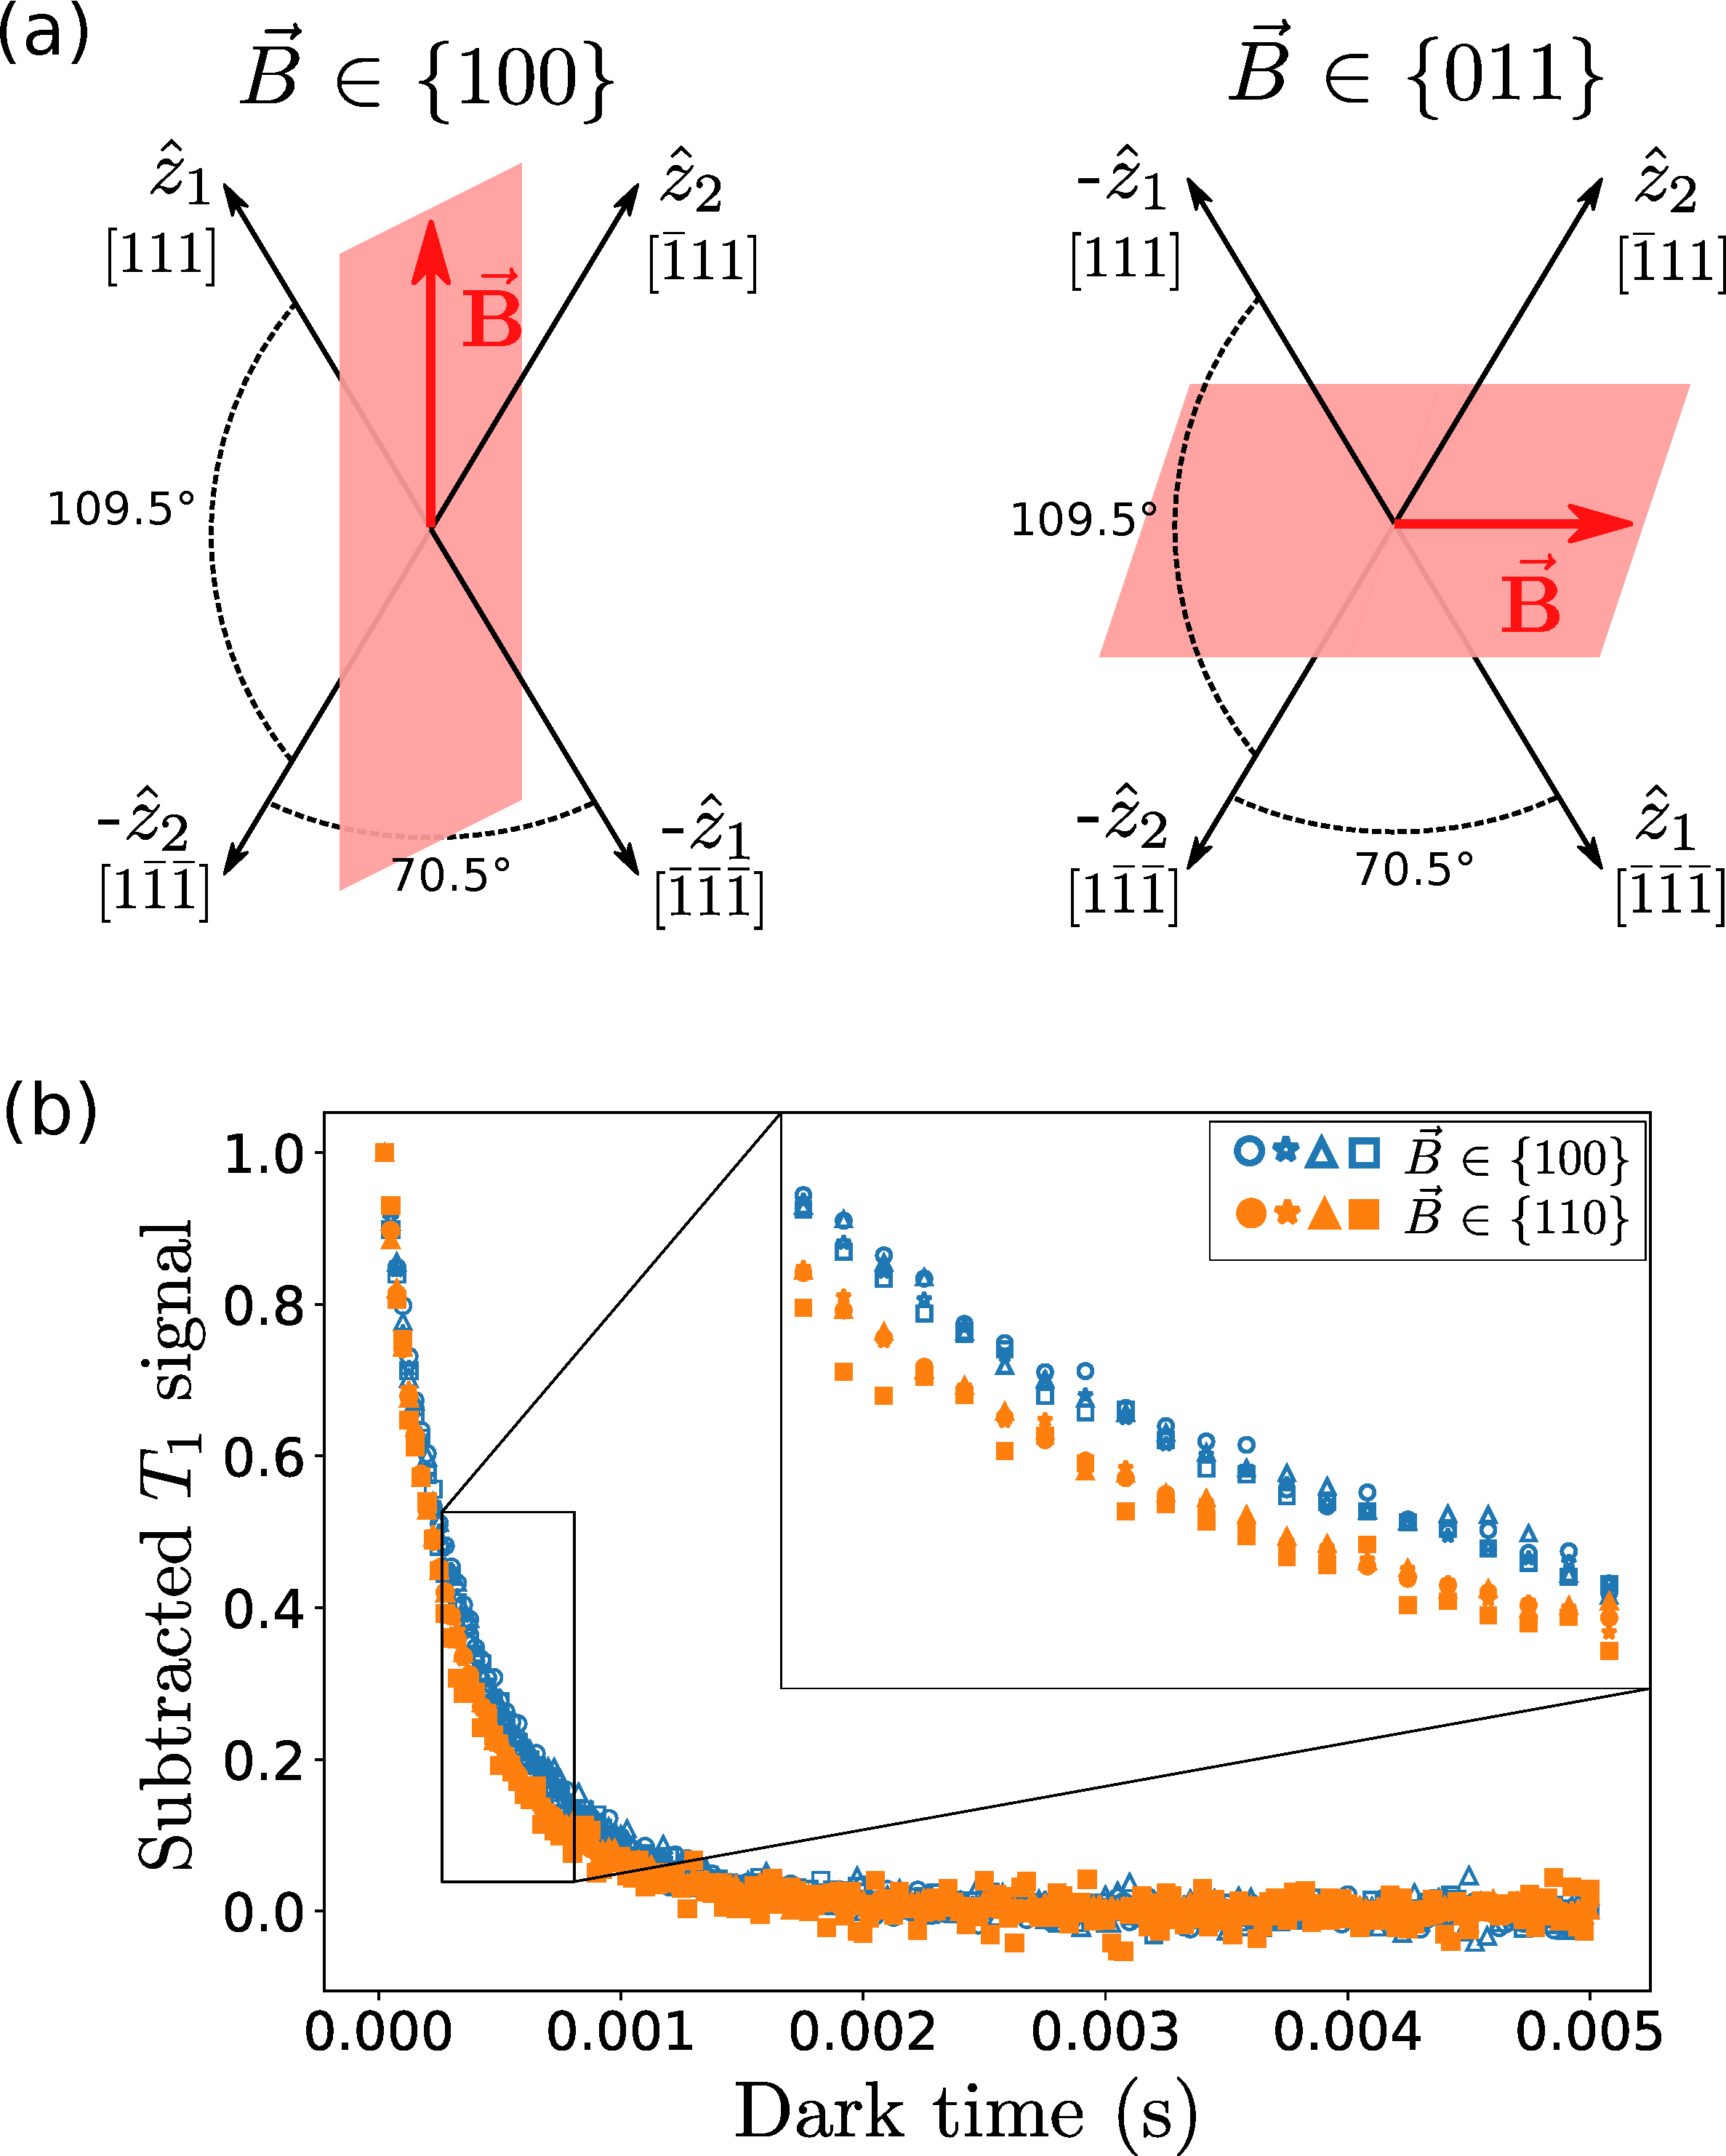
\includegraphics[width=0.7\textwidth]{Figures_SI/121_VS_22}
\caption{(a) Geometrical representation of two NV classes and the two possible planes where the magnetic field has the same projection on both classes. The positive $\hat z_i$ direction is chosen so that $\bm{B}\cdot \hat{z}_i >0$. (b) $T_1$ measurement on a two-class resonance following the protocol described in main text. 8 different magnetic field were used on the same sample : 4 times in a \{100\} plane (blue unfilled symbols) and 4 times in a \{110\} plane (orange filled symbols). Inset : zoom-in on the 0.3-0.8 ms region.}
\label{121 VS 22 fig}
\end{figure}

With these hypothesis, we found that there were 3 possible scenarios where the NV and fluctuator were resonant:
\begin{itemize}
\item The NV and fluctuator are resonant and from the same class (the angle $\widehat{z_1 z_2}=0$) : this is always true, regardless of the magnetic field. We can analytically compute $\bar \eta$ in this case and find : $$ \bar {\eta}_{same}=\frac{1}{4}  \int_\theta \int_\phi \abs{\eta(\bm u,\widehat{z_1 z_2}=0,\omega_{NV}=\omega_f)}\, d\Omega= \frac{1}{4} \cdot \sqrt{\frac{1}{3}} \cdot \frac{2}{3 \sqrt{3}} \approx 5.55\cdot10^{-2}$$
\item The NV and fluctuator are resonant and the angle $\widehat{z_1 z_2}=\rm{arccos}(\frac{1}{3})\approx 70.5^\circ$. This happens when the magnetic field lies in the \{100\} crystalline planes family. In this case we can numerically compute $\bar \eta_{\rm close} \approx \frac{1}{4} \cdot \sqrt{\frac{1}{3}} \cdot 0.6507 \approx 9.39\cdot10^{-2}$
\item The NV and fluctuator are resonant and the angle $\widehat{z_1 z_2}=\rm{arccos}(-\frac{1}{3})\approx 109.5^\circ$. This happens when the magnetic field lies in the \{110\} or \{$1\bar{1}0$\} crystalline planes family. In this case we can numerically compute $\bar \eta_{\rm far} \approx \frac{1}{4} \cdot \sqrt{\frac{1}{3}} \cdot 0.8328 \approx 1.20\cdot10^{-1}$. This last case was not taken into account by \cite{choi_depolarization_2017}.
\end{itemize}



Fig. \ref{121 VS 22 fig}(a) shows a graphical representation of the difference between the two last scenarios : due to the $\bm{B}\cdot \hat{z} >0$ condition, the same two classes of NV centers can have a $\widehat{z_1 z_2}$ angle equal to $70.5^\circ$ or $109.5^\circ$ depending on the external magnetic field. 

These computed values can be tested experimentally. Fig. \ref{121 VS 22 fig}(b) shows the subtracted $T_1$ signal measured on the same sample HPHT-15-2 for 8 different values of the magnetic field, each time on a two-class resonance : in 4 cases the magnetic field was in a \{100\} plane, and in the 4 other cases it was in a \{110\} plane. We can see that the measured lifetime is always smaller on the \{110\} case, which corresponds the the greater $\bar \eta$ factor computed previously.

\begin{figure}
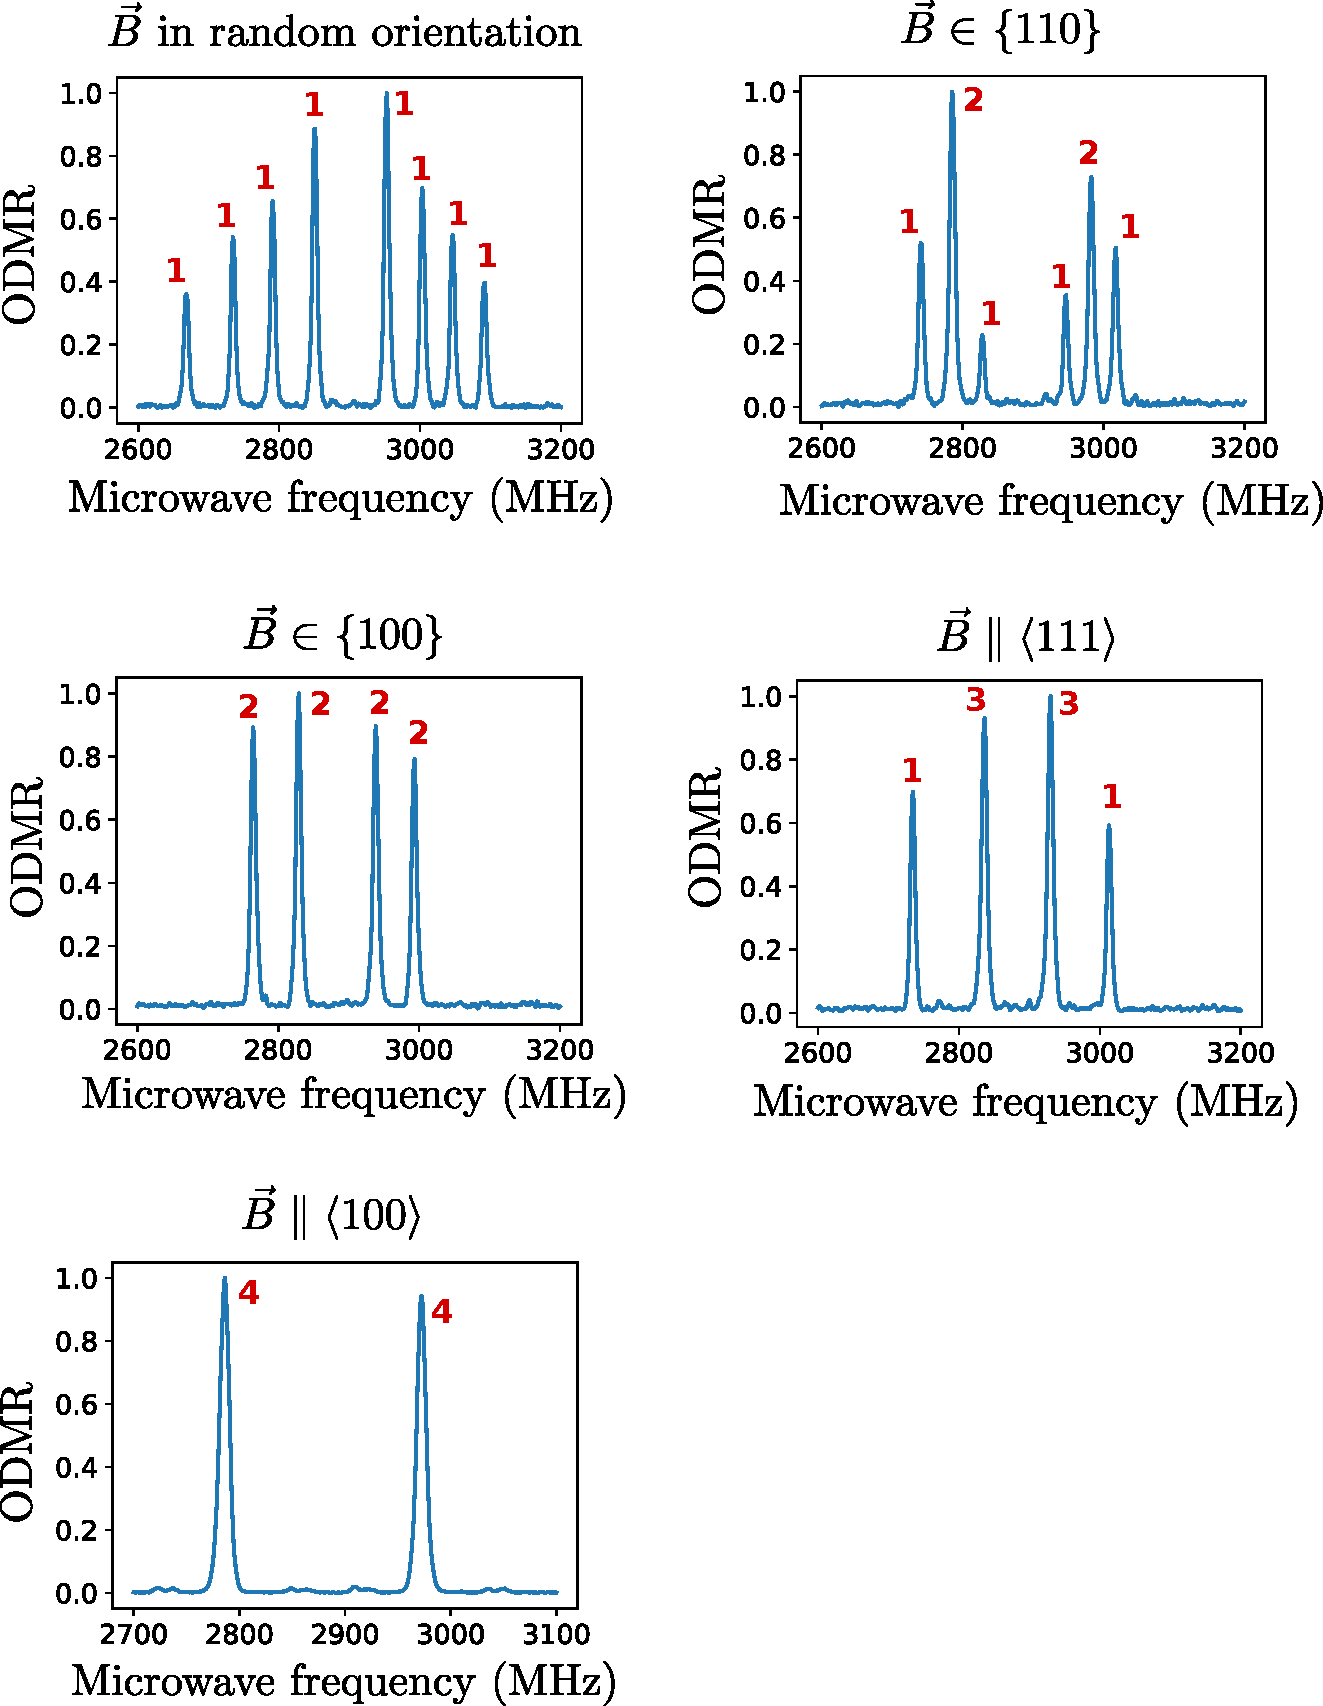
\includegraphics[width=0.7\textwidth]{Figures_SI/Various_ESR}
\caption{ODMR spectra for different orientations of the magnetic field. Red numbers represent the number of degenerated classes for each line of the spectrum}
\label{Various ODMR}
\end{figure}

Here is a list of the computed values of $\bar \eta^2$, which according to eq.(\ref{eq 1/T}) is proportional to the dipole induced decay rate, for various magnetic field orientation. An ODMR spectrum for each of these situations is present in Fig. \ref{Various ODMR}.
\begin{itemize}
\item Random orientation / no class degeneracy : for all four classes, $\bar \eta = \bar {\eta}_{\rm same}$ and $\bar \eta^2=3.08 \cdot 10^{-3} \equiv \bar \eta_0^2$
\item $\bm{B} \in$ \{110\} : For the two non resonant classes : $\bar \eta = \bar {\eta}_{\rm same}$ and $\bar \eta^2= \bar \eta_0^2$.  For the two resonant classes : $\bar \eta = \bar {\eta}_{\rm same} + \bar {\eta}_{\rm far}$ and $\bar \eta^2\approx\, 10.0 \bar \eta_0^2$
\item $\bm{B} \in$ \{100\} : For each pair of two-classes resonance: $\bar \eta = \bar {\eta}_{\rm same}+\bar {\eta}_{\rm close}$ and $\bar \eta^2\approx 7.24\, \bar \eta_0^2$. 
\item $\bm{B} \parallel \langle 111 \rangle$ : For the non-resonant class (parallel to $\bm B$) : $\bar \eta = \bar {\rm \eta}_{same}$ and $\bar \eta^2= \bar \eta_0^2$. For the triply resonant classes: $\bar \eta = \bar {\eta}_{\rm same}+2\bar {\eta}_{\rm far}$ and $\bar \eta^2\approx 28.4\, \bar \eta_0^2$. 
\item $\bm{B} \parallel \langle 100 \rangle$ : For the quadruple resonance : $\bar \eta = \bar {\eta}_{\rm same}+2\bar {\eta}_{\rm close} + \bar {\eta}_{\rm far}$  and $\bar \eta^2\approx 42.8\, \bar \eta_0^2$.
\end{itemize}

The measured increase in the decay rate is generally smaller than the predicted one : we measured an increase by a factor $\sim 4$ for a two-class degeneracy instead of the predicted $10.0$, and an increase by a factor $\sim 16$ for a four-class degeneracy instead of the predicted $42.8$. \cite{choi_depolarization_2017} measured an increase by a factor $\sim 4$ on a two-class degeneracy instead of the predicted $7.24$ or $10.0$.

\subsection{Flip-flops in the non-magnetic basis $\{ \ket{0},\ket{+},\ket{-} \} $}

As described in sec. \ref{sec Hamiltonian}, when the single spin Hamiltonian of the NV center is dominated by the electric field or the transverse magnetic field (as long as $\gamma_e B_\perp \ll D$), the eigenbasis of the NV Hamiltonian is close to $\{\ket{0},\ket{+}=\frac{\ket{+1}+\ket{-1}}{\sqrt{2}},\ket{-}=\frac{\ket{+1}-\ket{-1}}{\sqrt{2}} \} $. We therefore have to rewrite the dipole-dipole Hamiltonian using this new basis for both spins in order to perform similar calculations as the ones done in the previous section.

Since the flip-flop processes are now of the form $\ket{0,\pm}\bra{\pm,0}$, we redefine the $\eta$ factor as :
\begin{equation}
\eta^2=\frac{1}{3} \abs{\mel{\pm ,0}{\frac{\mathcal{H}_{\rm dd}}{J_0/r^3}}{0,\pm }}^2  \frac{4\gamma_f^2}{(\omega_f - \omega_{NV})^2+4\gamma_f^2}
\end{equation}

In this new basis, the spin operators are written :

\begin{equation}
  S_x = \begin{pmatrix}
  0&1&0 \\
  1&0&0 \\
  0&0&0
  \end{pmatrix}
  \begin{matrix}
  \bra{-} \\
  \bra{0} \\
  \bra{+}
  \end{matrix}  
  , \quad 
 S_y = \begin{pmatrix}
  0&0&0 \\
  0&0&1 \\
  0&1&0
  \end{pmatrix}
  \begin{matrix}
  \bra{-} \\
  \bra{0} \\
  \bra{+}
  \end{matrix}  
 , \quad 
  S_z = \begin{pmatrix}
  0&0&1 \\
  0&0&0\\
  1&0&0
  \end{pmatrix}
  \begin{matrix}
  \bra{-} \\
  \bra{0} \\
  \bra{+}
  \end{matrix}
  \end{equation}

The symmetry in the $(xy)$ plane is broken by the presence of the transverse electric or magnetic field. The $x_i$ direction is defined as the direction of the transverse electric or magnetic field which dominates the single spin Hamiltonian of the particle $i$.

We will consider two cases :
\begin{itemize}
\item The $x$ direction is defined by an external field (transverse magnetic field or strong external electric field) projected on the $(xy)$ plane of each classes. In particular this means that two spins from the same class have the same $(\hat x, \hat y, \hat z)$ basis.
\item The $x$ direction is defined by the local electric field generated by the charges in the crystal. We will assume that there are no correlations in the electric field between the NV and fluctuator, and will sample a random angle $\psi \in [0,2\pi]$ between the axes $\hat{x}_1$ and $\hat{x}_2$.
\end{itemize}

\begin{table}
\begin{tabular}{cccc}
\hline
$\bar{\eta}$ table & $\widehat{z_1 z_2}=0$ & $\widehat{z_1 z_2}=70.5^\circ$ & $\widehat{z_1 z_2}=109.5^\circ$ \\
\hline
$\ket{\pm 1}$ basis & $\frac{2}{3\sqrt{3}}=$ 0.3849 & 0.6507 & 0.8328 \\
$\ket{+/-}$ basis $\hat{x}_1\neq \hat{x}_2$ & 0.7110  & 0.6828 & 0.6828 \\
$\ket{+/-}$ basis $\hat{x}_1= \hat{x}_2$ & $\frac{4}{3\sqrt{3}}=$0.7698  & 0.6951 & 0.6951 \\
\hline
\end{tabular}
\caption{Computation of $\frac{\bar{\eta}}{ \frac{1}{4} \cdot \sqrt{\frac{1}{3}}}$ for the different eigenbasis of the single spin Hamiltonian, and for the different angles between the $z$ axis of the two spins.}
\label{table eta}
\end{table}

For this two cases, which we will call $\hat{x}_1=\hat{x}_2$ and $\hat{x}_1\neq \hat{x}_2$, we can compute the $\bar \eta$ factor for the three scenarios discussed previously : $\widehat{z_1 z_2}=0$ (same class), $\widehat{z_1 z_2}=70.5^\circ$ and $\widehat{z_1 z_2}=109.5^\circ$. The results, as well as those in the $\ket{\pm 1}$ basis are presented in Table \ref{table eta}.

There are two particular situations where these values can be experimentally tested :

The first one is described in Fig. 4 of the main text : in the presence of pure transverse magnetic field (for a single class, non-resonant with the three other classes), the decay rate of the class decreases with the magnetic field amplitude, due to the double-flip processes (described below), and then reaches a plateau with a decay rate value $\sim 2$ times bigger than in the longitudinal magnetic field case. This increase is in agreement with the fact that $\bar{\eta}_{\rm same}$ is 2 times bigger in the non-magnetic $\ket{+/-}$ basis than in the magnetic $\ket{\pm 1}$ basis. The measured increase is again smaller than the predicted factor of 4 given by eq. (\ref{eq 1/T}).

The second one is the difference between the $\bm{B} \parallel \langle 100 \rangle$ case and the $\bm{B}=0$ case. When a magnetic field is applied in the [100] direction, all four classes are resonant and the spin Hamiltonian basis is $\{ \ket{0},\ket{+1},\ket{-1} \} $. The $\bar \eta$ factor in this case has been calculated in the previous section : $\bar \eta^2\approx 42.8\, \bar \eta_0^2$. When no external magnetic field is applied, all four classes are also resonant but the spin Hamiltonian basis is  $\{ \ket{0},\ket{+},\ket{-} \} $ (see Sec. \ref{NV Hamiltonian}) and double-flip processes are near-resonant. The decay rate due purely to flip-flop in the $\ket{+/-}$ basis is proportional to $\bar \eta^2 = (\bar{\eta}_{\rm same}^{+/-} + 3\bar{\eta}_{\rm diff}^{+/-})^2 \approx 51.4\, \bar \eta_0^2$. Fig. 3 of the main text shows that we indeed observe a shorter lifetime when $\bm B=0$, in agreement with the higher value of $\bar \eta^2$, but this decrease could also come from the double-flip processes which are absent when $\bm B \neq 0$.

\subsection{Double-flip processes}

Double-flip processes are processes where both spins lose or gain one unit of spin angular momentum, as ooposed to flip-flop processes where one spin loses one quantum and the other gains one. These are related to matrix elements  such as $\mel{+1,0}{\frac{\mathcal{H}_{\rm dd}}{J_0/r^3}}{0,-1}$ in the $\ket{\pm 1}$ basis or $\mel{+,0}{\frac{\mathcal{H}_{\rm dd}}{J_0/r^3}}{0,-}$ in the $\ket{\pm}$ basis. These matrix elements couple two-spin states that are never fully resonant, however with low-to zero magnetic, the residual splitting due to local electric and magnetic field ($\sim 6\ \rm MHz$ with our samples) is small enough compared to the fluctuators linewidth  measured in sec. \ref{fluctuator width} to be $\sim 8\ \rm MHz$, so that double-flip processes may still occur.

Fig. 4 of the main text shows that for lower transverse field values, the spin decay rate is increased significantly. We attribute this increase to double-flip processes. We can see that the decay rate increase ($\sim$ 5 times the baseline value) is significantly higher than the increase due solely to the $\ket{+/-}$ basis ($\sim$ 2 times the baseline value). This lead us to believe that the double-flip process are the main reason behind the decrease in spin lifetime for $\bm B=0$ observed in Fig. 4 of the main text. This would probably mean that double-flip processes are the dominant factor in the sensitivity of the magnetometry protocol presented in the main text.
\bibliographystyle{plain}

\bibliography{CR_SI}{}
\end{document}
